\section{Segunda consigna: gráficos y análisis}
%Aparte de los gráficos detallados en este informe existe una carpeta llamada ”grafos” donde se pueden visualizar los grafos de cada red analizada.

\subsection{Red con información previa}

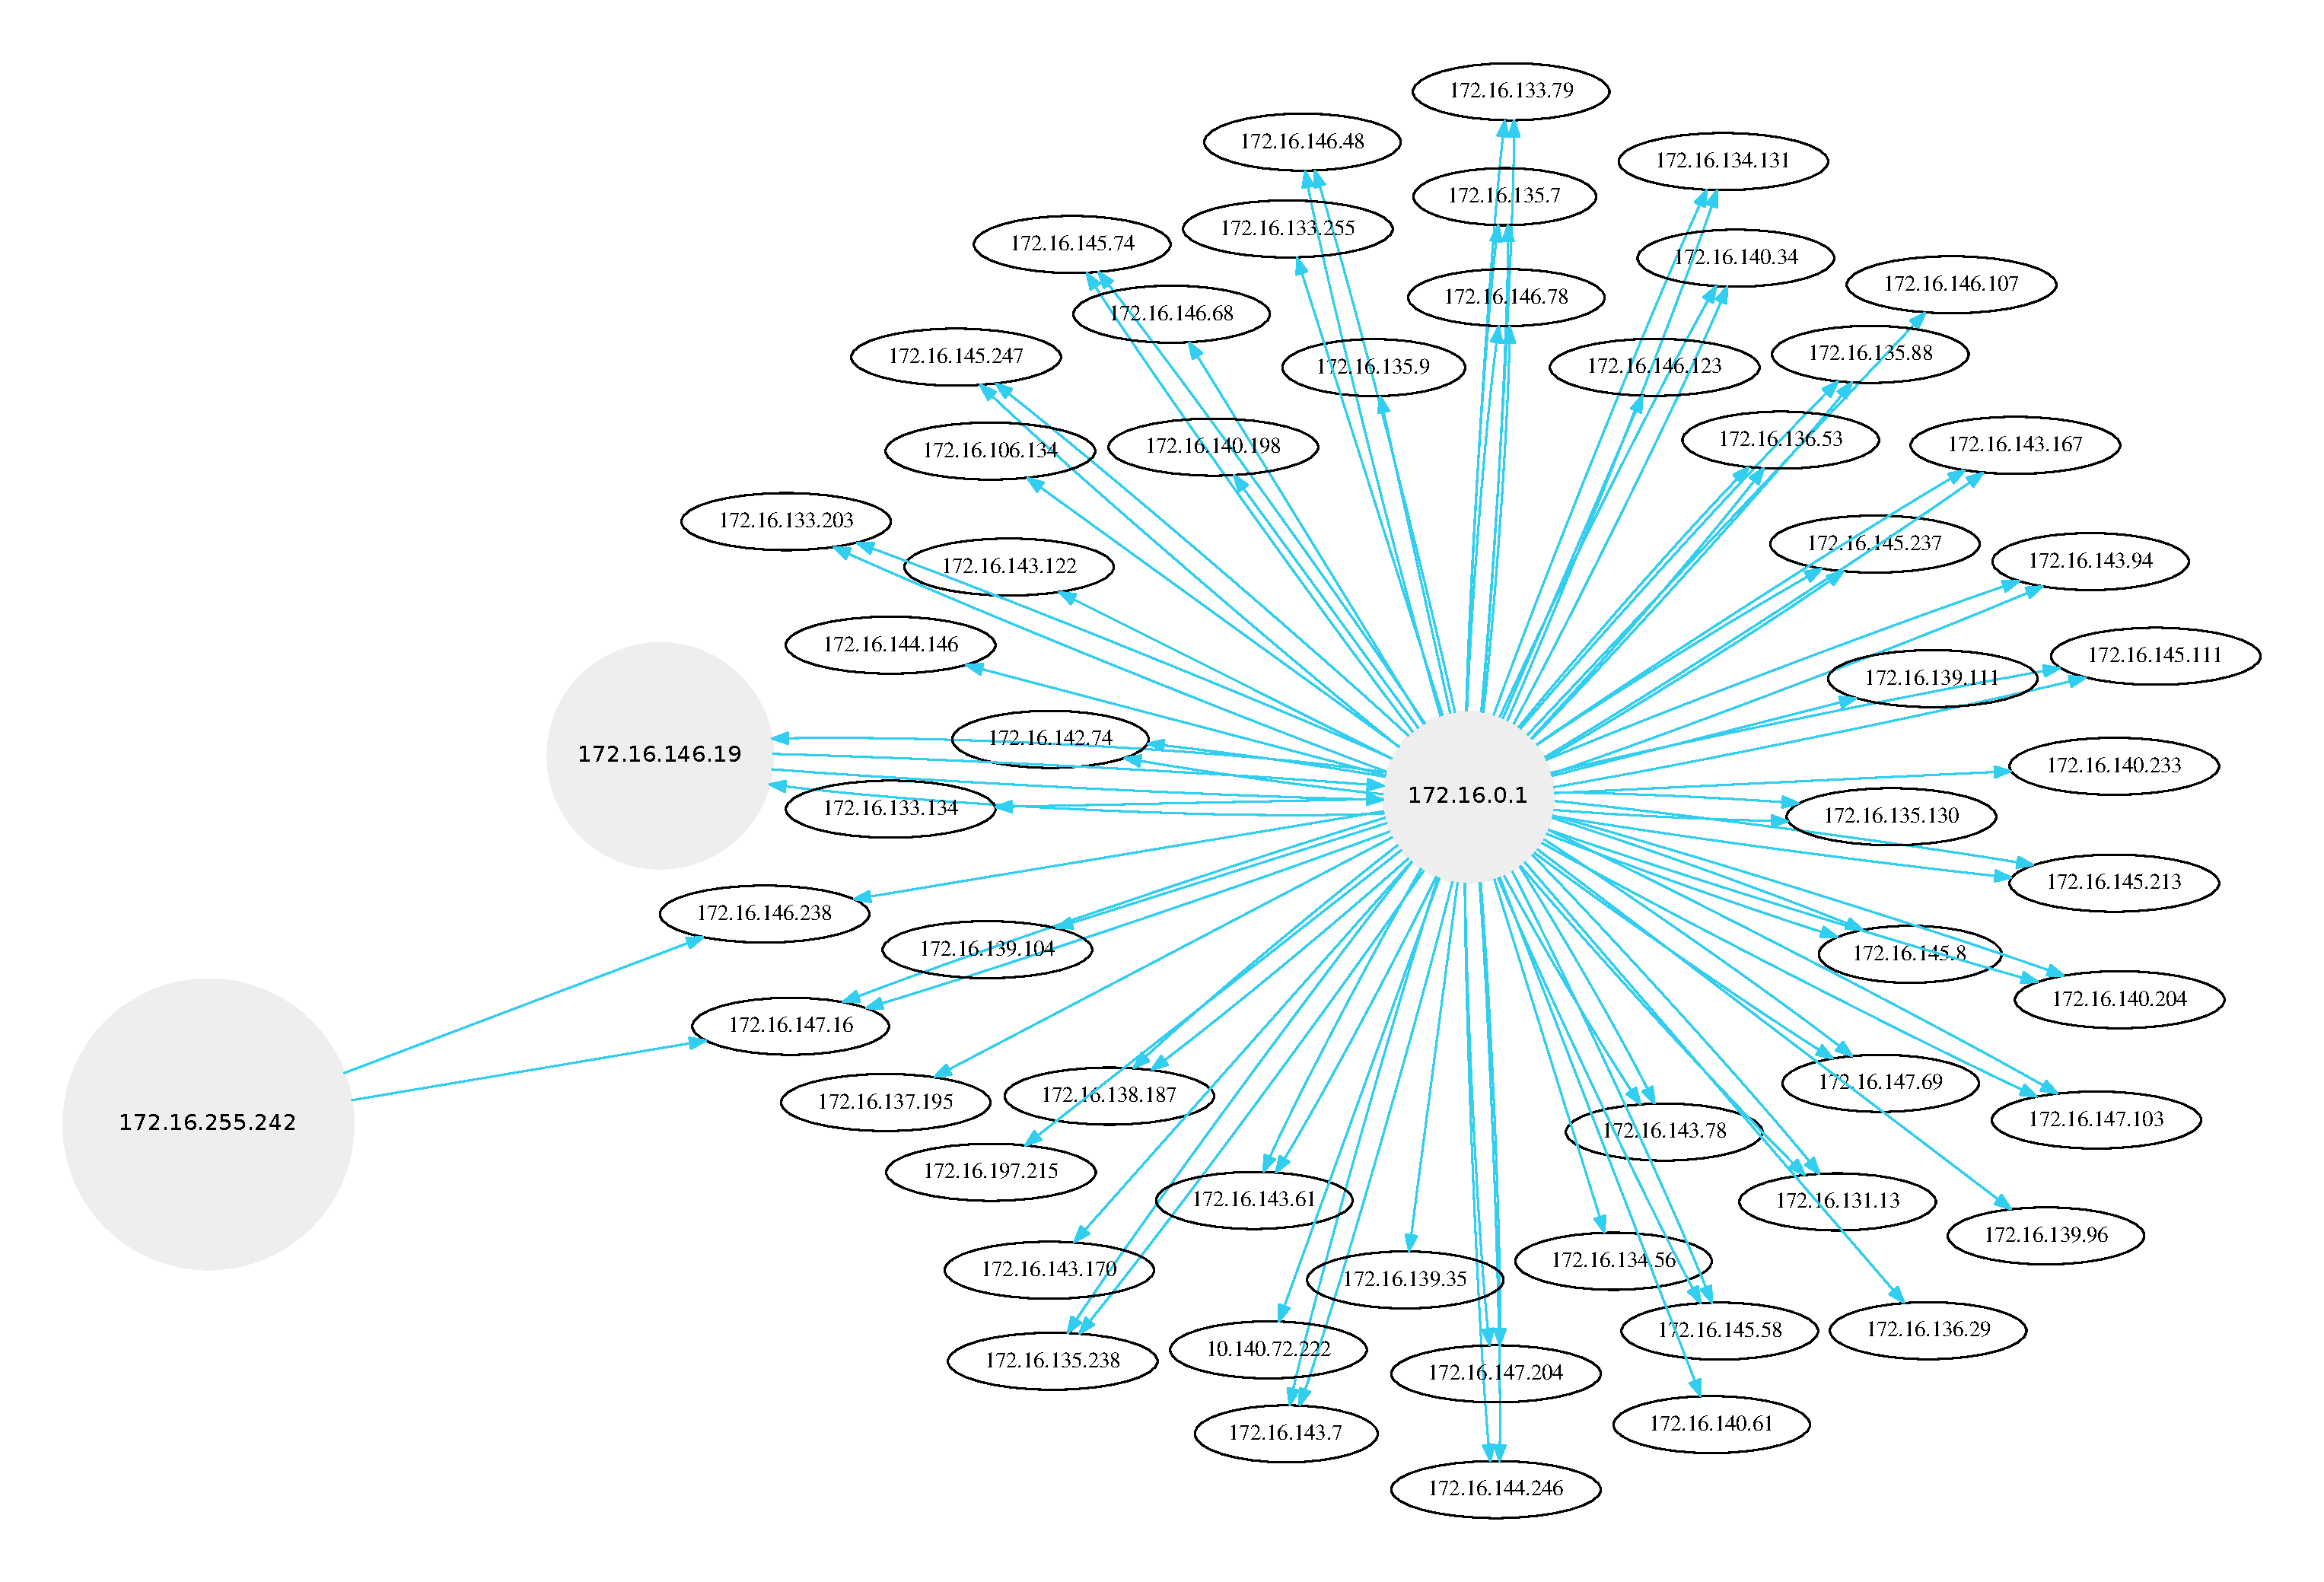
\includepdf[pages={1}]{abasto_grafo.pdf}


Para tener una base de partida sólida sobre la cual extrapolar, la primera captura que realizamos fue en una red hogareña de uno de los integrantes 
del grupo en la que cual pudieramos determinar de manera feaciente cada uno de los dispositivos que se encontraban en la red. Suponemos que el host
con una mayor interacción en envíos y recepción de paquetes $ARP$ será el router dado que todos los dispositivos buscarían comunicarse directamente
con él para acceder a Internet. Con respecto los demás dispositivos suponemos una interacción distribuida, donde se envían espacialmente paquetes $ARP$
en caso de querer establer alguna conexión o actualizar sus datos.\\

Durante la escucha, cada uno de los dispositivos concervó la siguente ip:\\
\begin{table}[htb]
\begin{center}
\begin{tabular}{|l|l|}
\hline
IP & Host \\
\hline \hline
192.168.1.1 & Router \\ \hline
192.168.1.3 & Celular (wifi) \\ \hline
192.168.1.6 & Computadora (wifi)  \\ \hline
192.168.1.10 & Computadora (wifi) \\ \hline
192.168.1.36 & Computadora (cable ethernet) \\ \hline
\end{tabular}
\caption{Información previa - Red Doméstica}
\label{tabla informacion}
\end{center}
\end{table}

%192.168.1.1 -> ip del router
%192.168.1.3 -> ip de celular (wifi)
%192.168.1.6 -> ip de mi computadora (wifi)
%192.168.1.36 -> computadora conectada por cable ethernet
%192.168.1.10 -> computadora conectada (wifi) con Windows 7

Lo que pudimos observar simulando la fuente $S$ durante $4$ horas en esta red fue lo siguiente:\\
%\begin{figure}[h!]
\centering
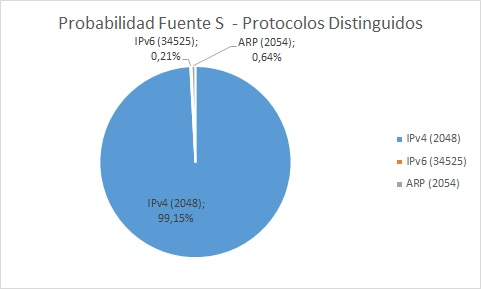
\includegraphics[width=\textwidth]{./img/probaS_casa.jpg}
\caption{Protocolos Distinguidos - Fuente S - Hogar}
\end{figure}
\newpage

\begin{figure}[h!]
\centering
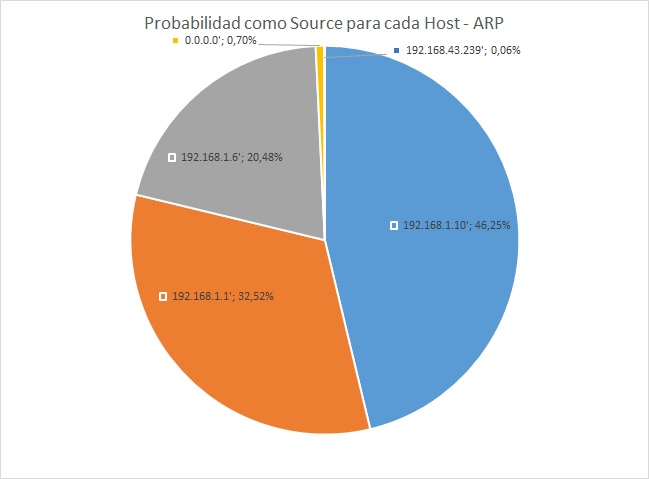
\includegraphics[width=\textwidth]{./img/proba_src_casa.jpg}
\caption{Probabilidad Source - Fuente S1(ARP) - Hogar}
\end{figure}

\begin{figure}[h!]
\centering
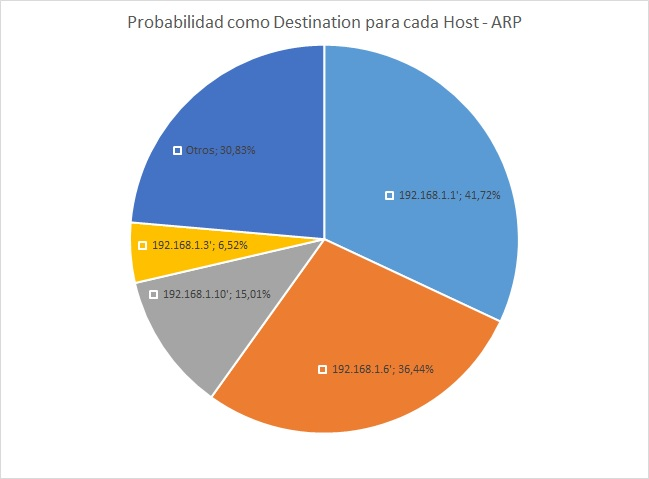
\includegraphics[width=\textwidth]{./img/proba_dst_casa.jpg}
\caption{Probabilidad Destination - Fuente S1(ARP) - Hogar}
\end{figure}
\newpage

\begin{figure}[h!]
\centering
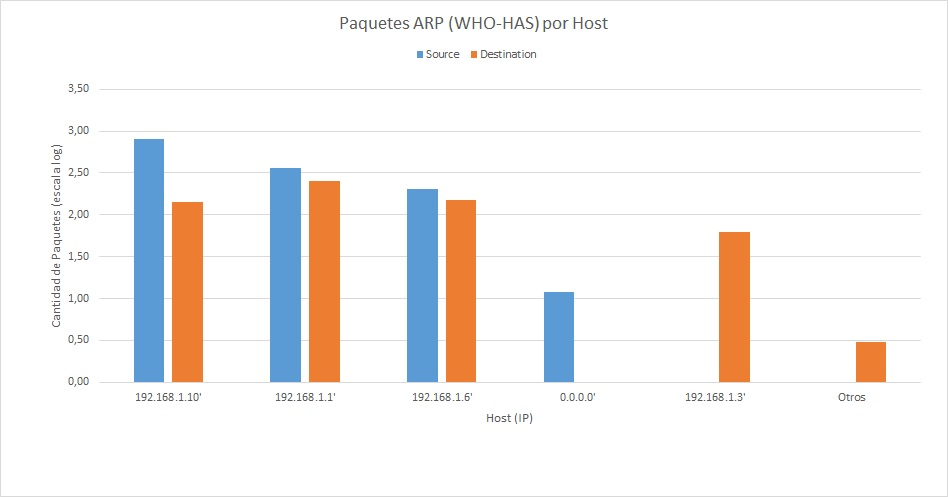
\includegraphics[width=\textwidth]{./img/arp_whoHas_casa.jpg}
\caption{Source/Destination paquetes ARP - Operación: Who-Has - Hogar}
\end{figure}

\begin{figure}[h!]
\centering
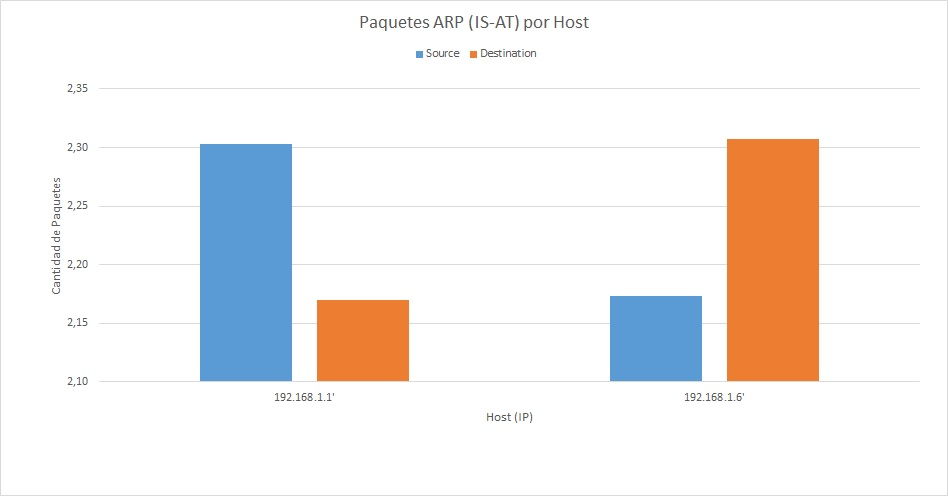
\includegraphics[width=\textwidth]{./img/arp_isAt_casa.jpg}
\caption{Source/Destination paquetes ARP - Operación: Is-At - Hogar}
\end{figure}


\newpage
\begin{figure}[h!]
\centering
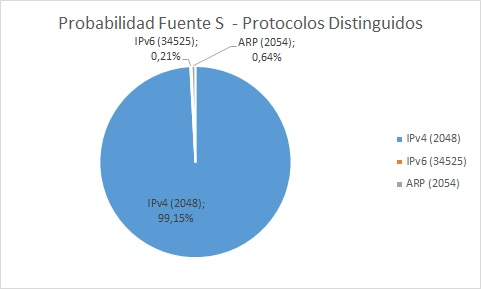
\includegraphics[scale=0.9]{./img/probaS_casa.jpg}
\caption{Protocolos Distinguidos - Fuente S - Hogar}
\end{figure}

De esta información, podemos concluir que el símbolo del protocolo $IPv4$ es mucho más probable que el símbolo del protocolo $ARP$ y que $IPv6$. 
Por lo que con lo que respecta a la fuente de información $S$, el símbolo $IPv4$ contiene mucha menos información comparado contra los otros dos. 
El cálculo de entropía de la fuente para estos datos es $0.0771$ lo que de manera intuitiva indica que la incertidumbre sobre el próximo símbolo 
de la fuente es muy baja dado que es muy probable que el próximo protocolo en aparecer sea $IPv4$.\\

Sobre la misma escucha, como ya adelantamos, simulamos la fuente de información $S1$. 
La entropía de la fuente $S1$ es de $1.98$. Esto nos parece más lógico, ya que en este caso hay más símbolos en el sistema y 
además cada uno tiene una probabilidad considerable de aparecer. Aunque, como ya veremos, algunos son más probables que otros.\\

Sobre la fuente $S1$, los resultados son los que se muestran en los siguientes diagramas:

\begin{figure}[h!]
\centering
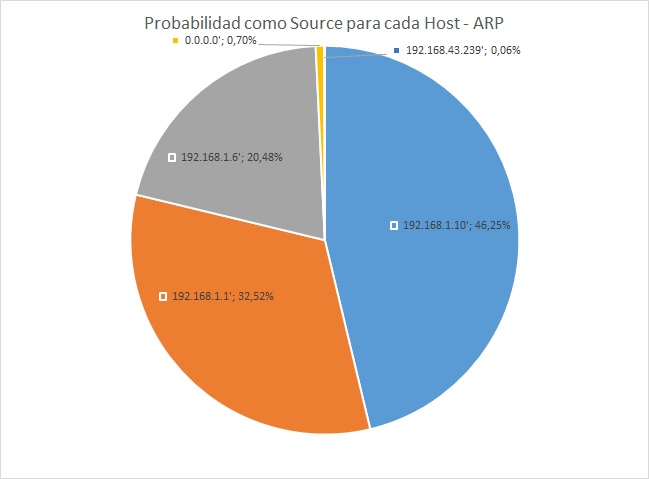
\includegraphics[scale=0.7]{./img/proba_src_casa.jpg}
\caption{Probabilidad Source - Fuente S1(ARP) - Hogar}
\end{figure}

\begin{figure}[h!]
\centering
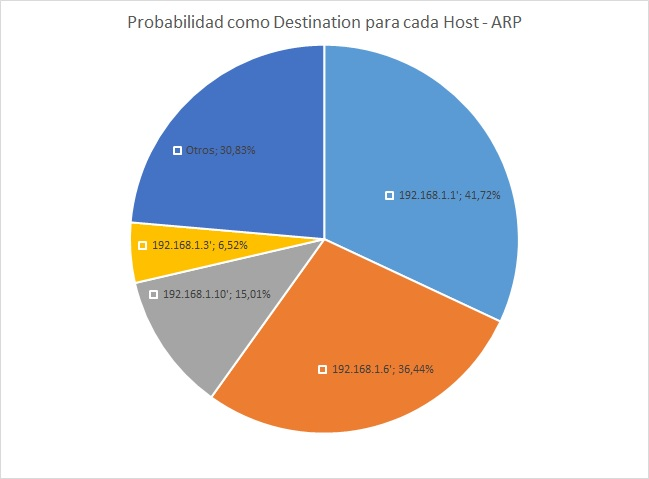
\includegraphics[scale=0.7]{./img/proba_dst_casa.jpg}
\caption{Probabilidad Destination - Fuente S1(ARP) - Hogar}
\end{figure}
\newpage

Sobre esta fuente se deben mencionar varias particularidades observadas que resultan interesantes:

\begin{itemize}
\item{La computadora con $IP$ asignada 192.168.1.10 en cierto momento realiza un escaneo sistemático de toda la red local, preguntando 
para cada ip dentro del rango 192.168.1.1-254 a quién pertenece la $MAC$. El equipo en cuestion es una computadora personal con Windows 7 instalado 
y nos resultó sorprendente observar este comportamiento para una computadora personal. 
La única explicación a la que pudimos llegar con respecto a esto es que la computadora se encuentra afectada por algún tipo de aplicación 
de bajo o alto nivel que intenta obtener información de la red local. No esperábamos este resultado este resultado para este dspositivo en particular.}

\item{Al preguntar algún host por la computadora con ip 192.168.1.36 (que se encuentra conectada por un cable ethernet al router) 
el router responde a la red wifi con su propia dirección $MAC$. En este sentido, el router estaría actuando como un bridge dentro de la red local.}

\item{El router (192.168.1.1) es el nodo que más se distingue dentro de la red. Es el que mayor interacción tiene en enviar y recibir 
paquetes $ARP$. Esto era de esperarse dado que es el host al que todos los otros preguntan dado que es el host a través del cuál 
todos los demás dispositivos acceden a Internet. El router necesita establecer y mantener actualizadas las direcciones $IP$ con las $MAC$ para
garantizar cierta fluidez en las comunicaciones.}

\end{itemize}

A continuación con toda la información obtenida, pueden observarse quiénes son los dispositivos que hacen más $Who-Has$ (azul) y 
cuáles son los dispositivos por los que más se hace $Request$ de $Who-Has$ (naranja):
\newpage

\begin{figure}[h!]
\centering
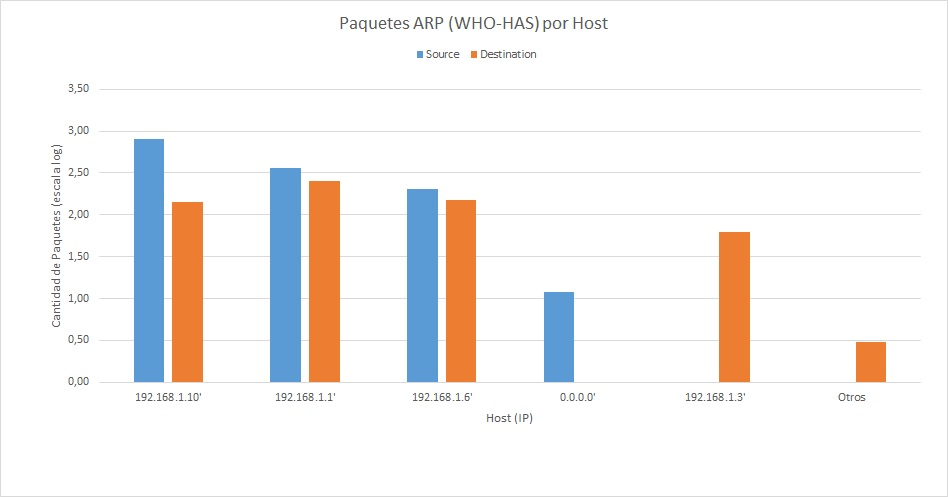
\includegraphics[scale=0.5]{./img/arp_whoHas_casa.jpg}
\caption{Source/Destination paquetes ARP - Operación: Who-Has - Hogar}
\end{figure}

De igual manera, cuáles son los que hacen más $Is-At$ (azul) y para quién está destinado el $Is-At$ (naranja):

\begin{figure}[h!]
\centering
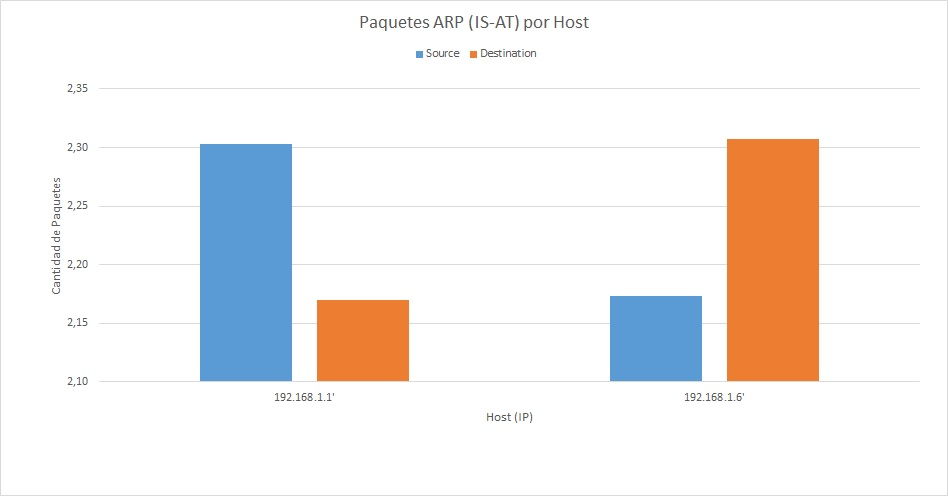
\includegraphics[scale=0.5]{./img/arp_isAt_casa.jpg}
\caption{Source/Destination paquetes ARP - Operación: Is-At - Hogar}
\end{figure}

De estos gráficos no ha llamado la atención el envío de paquetes $ARP$ de la $IP 0.0.0.0$. Son paquetes de operación $Whi-Has$ al host
192.168.1.10 solamente. También figura con una interacción alta la $IP$ 192.168.1.6 pero se debe comunicaciones con el router que le envía
continuamente paquetes $ARP$ consultado por su $MAC$ y la computadora 192.168.1.6 responde de manera automática. Esto también nos ha llamado la 
atención dado que si bien el router recibe la respuesta ($Is-At)$ del dispositivo hemos detectado que le sigue enviando $Who-Has$ para saber su $MAC$.\\

También observamos que el nodo 192.168.1.36 no envía paquetes $ARP$ al router, pero sabemos que esto es porque está conectada directamente
a él a través de un cable ethernet.\\

Por último, hemos generado el grafo de la red doméstica. En mismo se encuentra en la carpeta ”grafos” con el nombre $red\_domestica.png$. 
En dicho grafo se pueden visualizar los principales aspectos detallados anteriormente y nos permite entender mejor la relación entre cada 
dispositivo en cuánto al envío y recepción de los paquetes $ARP$.

\subsection{Redes sin información previa}
A continuación se muestra la cantidad de paquetes ARP por host en escala logarítmica. 
En el momento de realizar los gráficos, notamos que contabamos con una gran cantidad de hosts con muy baja probabilidad. 
Para mejorar la claridad y permitir apreciar los resultados a gran escala, decidimos filtrar estos casos y expresarlos como $Otros$ ya que 
no vimos valor en mostrar nodos con un 0,05 de probabilidad.\\

En las tres redes que se detallan a continuación nos hemos conectado por medio Wifi y son redes de espacios públicos sin seguridad. 
Por tal motivo cualquier dispositivo podría incorporarse a la red en cualquier momento.\\

\subsubsection{Probabilidad Protocolos - Fuente $S$}
A continuación mostramos los gráficos de Probabilidad de la fuente $S$ en las tres redes analizadas:

\begin{figure}[h!]
\centering
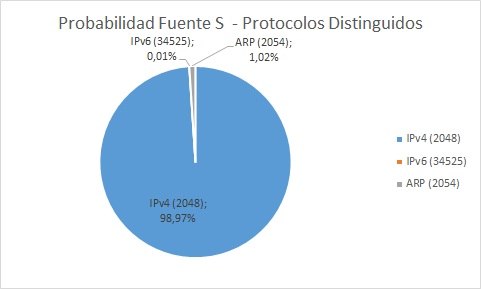
\includegraphics[scale=0.7]{./img/probaS_abasto.jpg}
\caption{Protocolos Distinguidos - Fuente S - Abasto}
\end{figure}

\begin{figure}[h!]
\centering
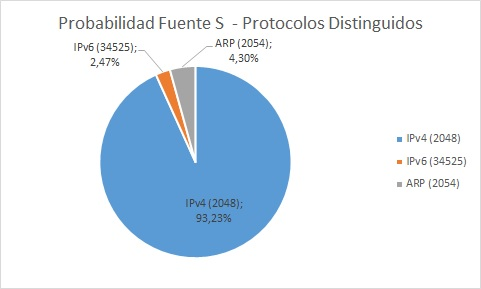
\includegraphics[scale=0.7]{./img/probaS_laboDC.jpg}
\caption{Protocolos Distinguidos - Fuente S - laboratoriosDC}
\end{figure}
\newpage

\begin{figure}[h!]
\centering
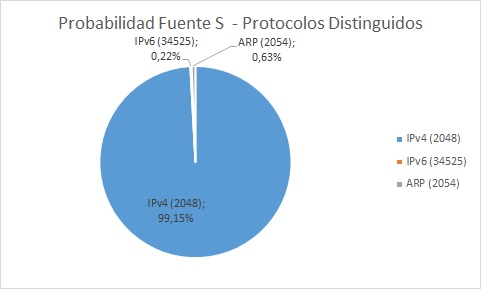
\includegraphics[scale=0.7]{./img/probaS_aulasDC.jpg}
\caption{Protocolos Distinguidos - Fuente S - aulasDC}
\end{figure}

\begin{table}[htb]
\begin{center}
\begin{tabular}{|l|l|}
\hline
Red & Entropía - Fuente $S$  \\
\hline \hline
Abasto & 0.0837 \\ \hline
laboratoriosDC & 0.4213 \\ \hline
aulasDC & 0.0774  \\ \hline
\end{tabular}
\caption{Entropía de cada Red analizada - Fuente $S$}
\label{tabla informacion}
\end{center}
\end{table}

En las redes $laboratoriosDC$ y $Abasto$ la probabilidad de paquetes con protocolo $ARP$ es mayor a la red doméstica estudiada anteriormente. 
Al ser redes abiertas y sin seguridad hay dispositivos saliendo e ingresando constantemente de las redes. Este motivo, sumado además a que 
son espacios públicos que cubren varios metros, produce que haya más paquetes $ARP$ para ir asignando la $IP$ con la $MAC$ correspondiente.
Curiosamente esto no se ha cumplido en la red $aulasDC$. Queriendo encontrar una respuesta suponemos que la mayoría de los dispositivos de la facultad
se esta conectando a la red $laboratoriosDC$ dado que en la práctica tiene un mejor señal. Al debatirlo, uno de los integrantes del grupo aclaró que
él se conectaba a la red $laboratoriosDC$ desde las aulas y que la misma tiene una mayor prioridad en su celular que $aulasDC$ para establecer 
conexión. Nos hemos basado en este caso para explicar este hecho que nos ha llamado la atención dado que esperábamos una mayor cantidad 
(en porcentaje) de paquetes $ARP$ en dicha red. Cuánto mayor es el porcentaje de los paquetes $ARP$ mayor es la entropía de las redes dado que 
no hemos detectado otros protocolos aparte de los tres detallados. Al haber más paquetes $ARP$ tenemos una mayor incertidumbre sobre el protocolo
del próximo paquete.\\

\newpage
\subsubsection{Fuente $S1$ - Paquetes $ARP$}

\textbf{Abasto Shopping}
\begin{figure}[h!]
\centering
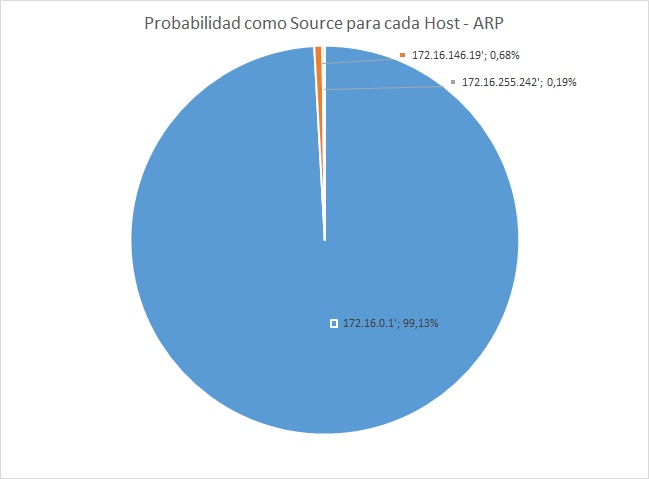
\includegraphics[scale=0.6]{./img/proba_src_abasto.jpg}
\caption{Probabilidad Source - Fuente S1(ARP) - Abasto}
\end{figure}

\begin{figure}[h!]
\centering
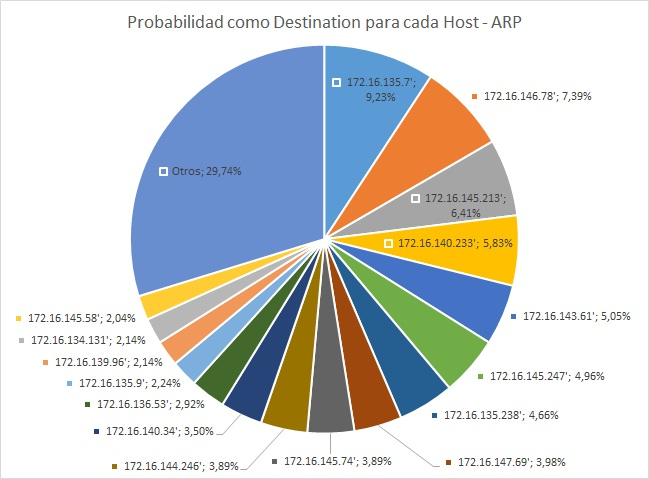
\includegraphics[scale=0.6]{./img/proba_dst_abasto.jpg}
\caption{Probabilidad Destination - Fuente S1(ARP) - Abasto}
\end{figure}
\newpage

\begin{figure}[h!]
\centering
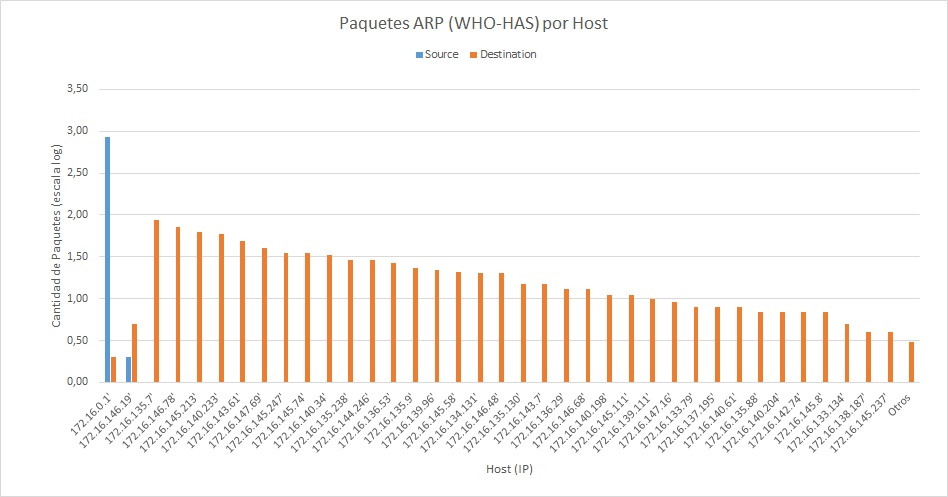
\includegraphics[scale=0.7]{./img/arp_whoHas_abasto.jpg}
\caption{Source/Destination paquetes ARP - Operación: Who-Has - Abasto}
\end{figure}

\begin{figure}[h!]
\centering
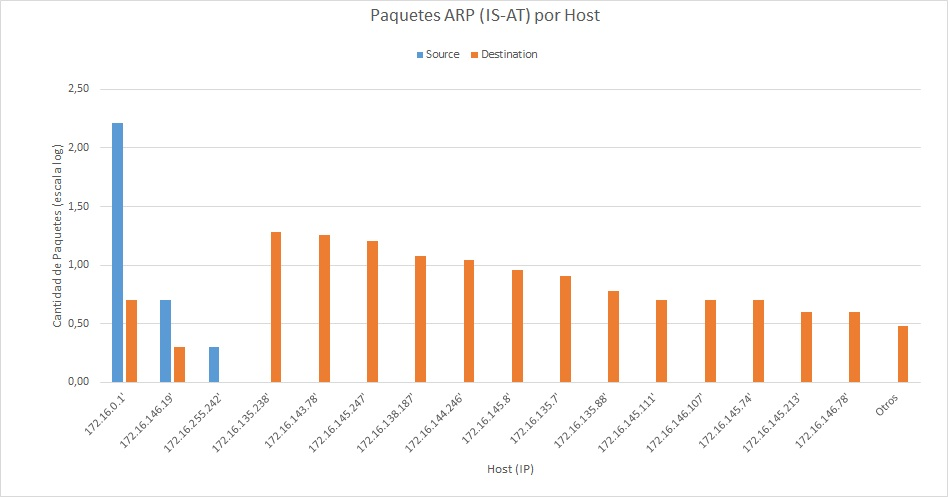
\includegraphics[scale=0.7]{./img/arp_isAt_abasto.jpg}
\caption{Source/Destination paquetes ARP - Operación: Is-At - Abasto}
\end{figure}
\newpage

\textbf{laboratoriosDC}
\begin{figure}[h!]
\centering
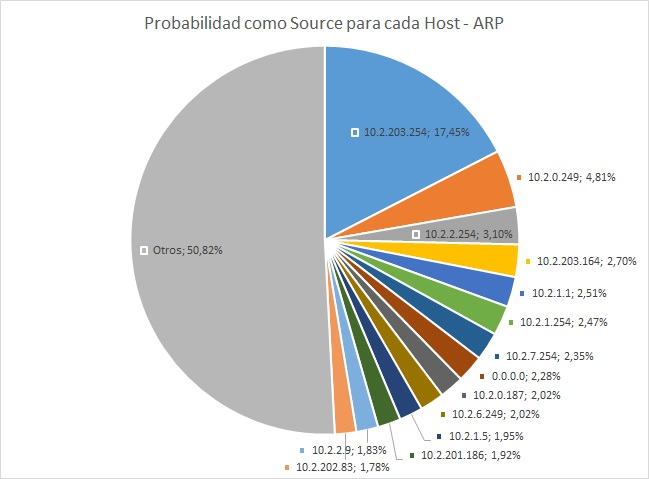
\includegraphics[scale=0.6]{./img/proba_src_laboDC.jpg}
\caption{Probabilidad Source - Fuente S1(ARP) - laboratoriosDC}
\end{figure}

\begin{figure}[h!]
\centering
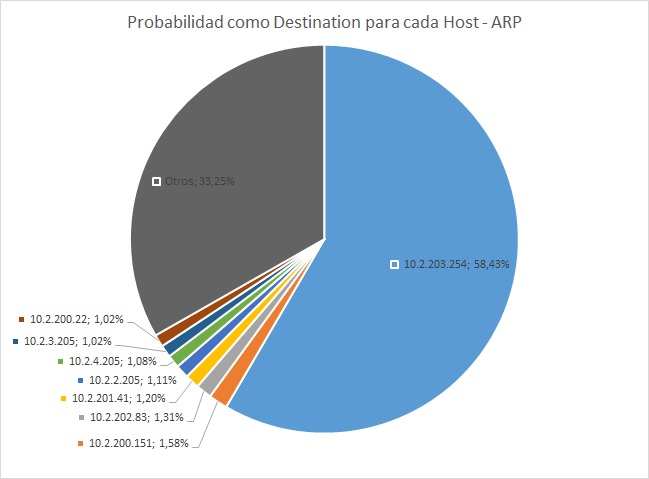
\includegraphics[scale=0.6]{./img/proba_dst_laboDC.jpg}
\caption{Probabilidad Destination - Fuente S1(ARP) - laboratoriosDC}
\end{figure}
\newpage

\begin{figure}[h!]
\centering
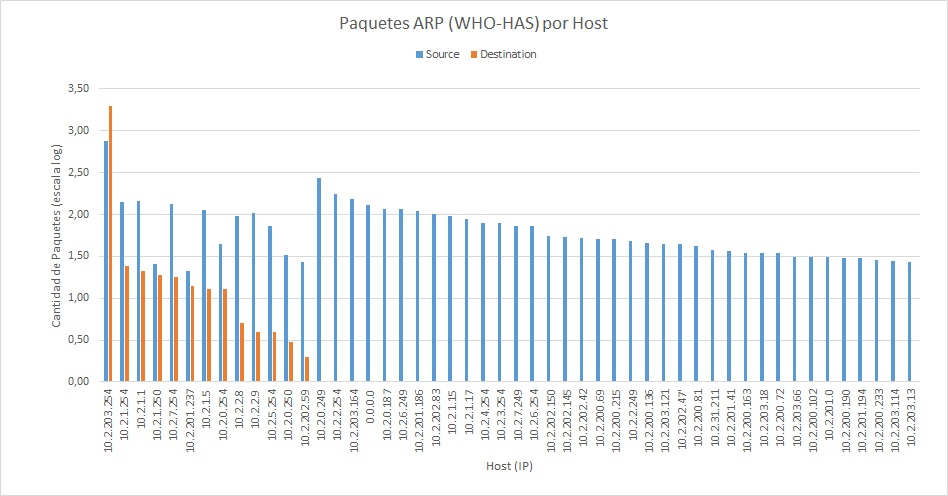
\includegraphics[scale=0.7]{./img/arp_whoHas_laboDC.jpg}
\caption{Source/Destination paquetes ARP - Operación: Who-Has - laboratoriosDC}
\end{figure}

\begin{figure}[h!]
\centering
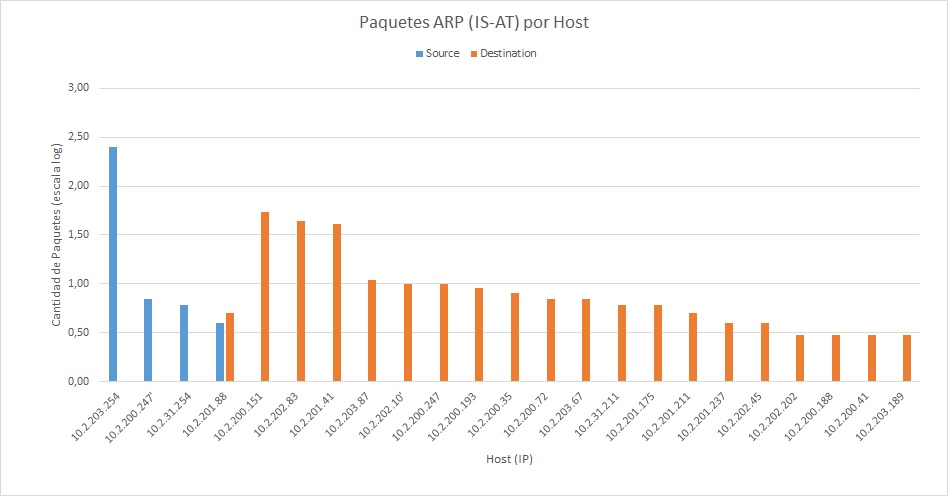
\includegraphics[scale=0.7]{./img/arp_isAt_laboDC.jpg}
\caption{Source/Destination paquetes ARP - Operación: Is-At - laboratoriosDC}
\end{figure}
\newpage

\textbf{aulasDC}
\begin{figure}[h!]
\centering
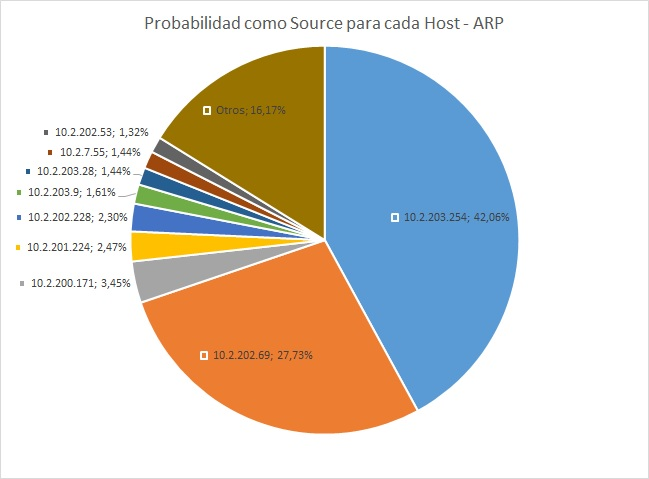
\includegraphics[scale=0.6]{./img/proba_src_aulasDC.jpg}
\caption{Probabilidad Source - Fuente S1(ARP) - aulasDC}
\end{figure}

\begin{figure}[h!]
\centering
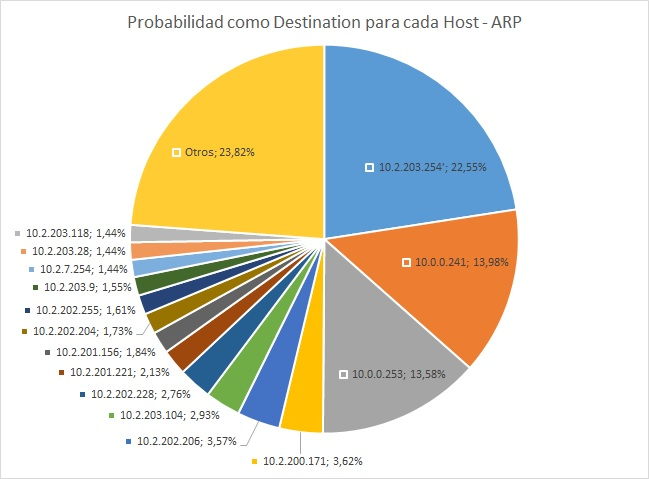
\includegraphics[scale=0.6]{./img/proba_dst_aulasDC.jpg}
\caption{Probabilidad Destination - Fuente S1(ARP) - aulasDC}
\end{figure}
\newpage

\begin{figure}[h!]
\centering
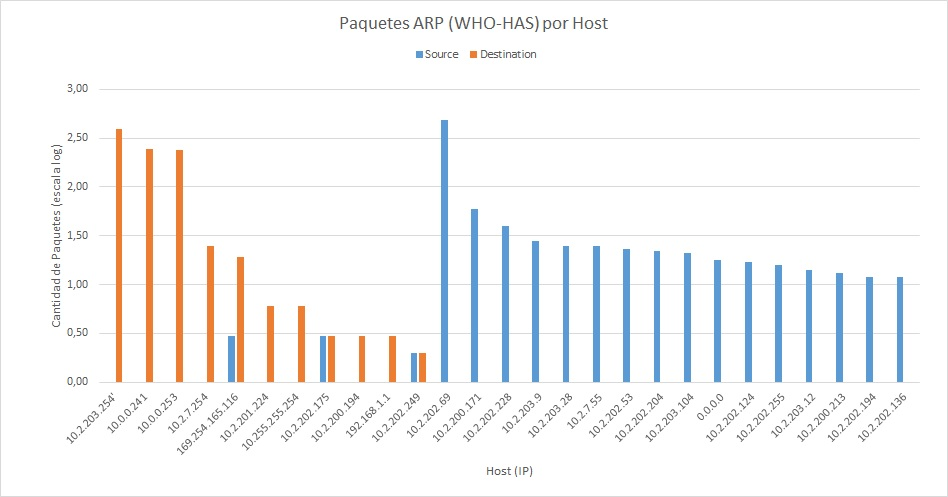
\includegraphics[scale=0.7]{./img/arp_whoHas_aulasDC.jpg}
\caption{Source/Destination paquetes ARP - Operación: Who-Has - aulasDC}
\end{figure}

\begin{figure}[h!]
\centering
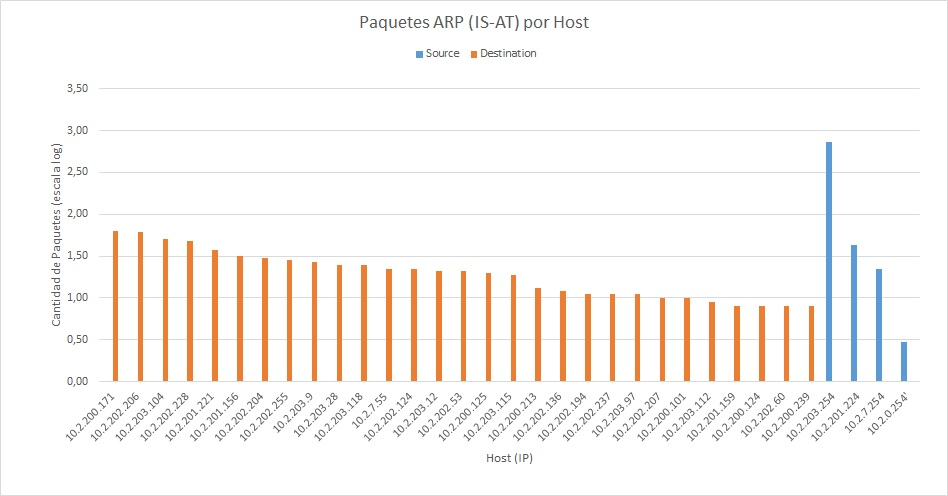
\includegraphics[scale=0.7]{./img/arp_isAt_aulasDC.jpg}
\caption{Source/Destination paquetes ARP - Operación: Is-At - aulasDC}
\end{figure}

Aca va frutaaaaaaaaa....